% subsection 4.6
\subsection{Stage 6: Results}
This section presents the results obtained through the execution of the SMS search protocol. Initially, a general description of the data corresponding to the Selected Primary Studies (SPSs) is provided.

This description covers aspects such as the origin of the studies, year of publication, search strategy, quality indices, their relationship with the research questions (RQs) and respective topics, and the keywords. Finally, a word cloud generated from the keywords of the SPSs is presented.

It is important to recall that the association between the SPSs and the topics was established through the detailed classification described in Section \ref{subsec:clasificacion-de-estudios}. Consequently, the RQs were also associated, since the topics follow a specific structure within them.

Furthermore, the association between the main SMS keywords and the section titles, abstracts, and keywords of all SPSs was identified.

% sub-subsection 4.6.1
\subsubsection{General Description of the SPSs (Selected Primary Studies)}
The process of searching and filtering studies resulted in the identification of 114 SPSs, as shown in Table \ref{table:selected_primary_studies}.

\begin{figure}[htbp]
	\centering
	\vspace{10pt}
	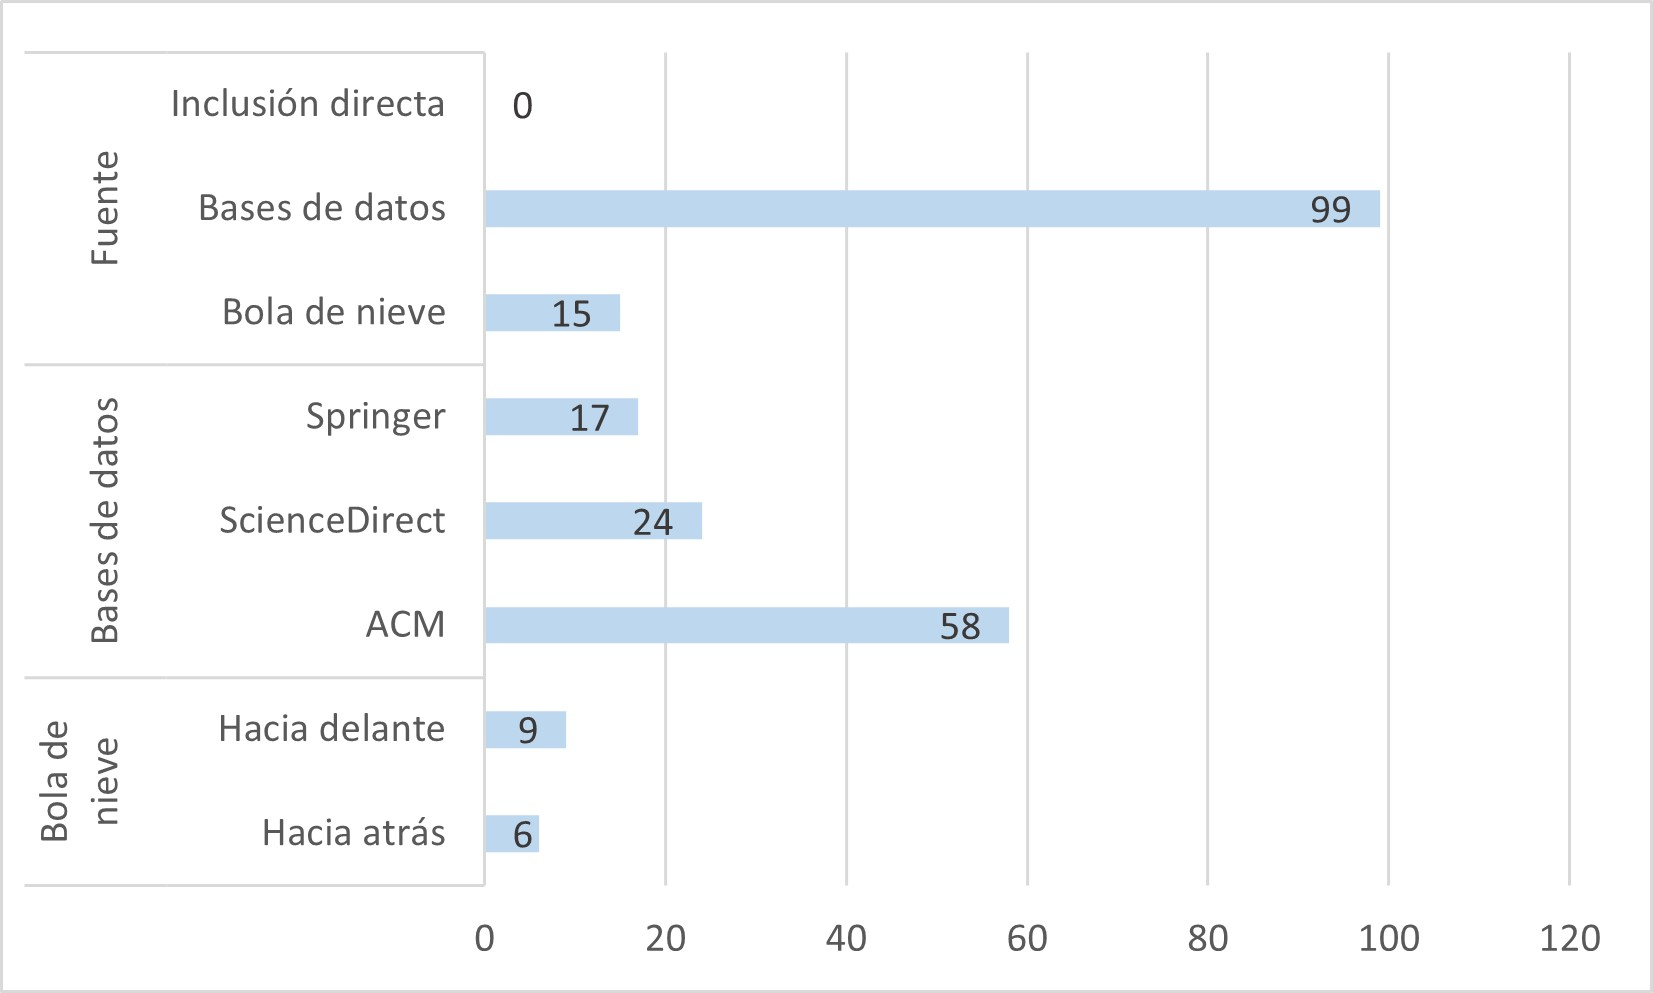
\includegraphics[scale=0.7]{resources/figures/SPSsByProcedence.jpg}
	\vspace{6pt}
	\caption{SPSs by source and search strategy.}
	\label{fig:SPSsByProcedence}
\end{figure}

These SPSs were obtained from digital databases, identified in the SMS through different strategies. Figure \ref{fig:SPSsByProcedence} shows the number of studies retrieved from various sources and the details of the database search and snowballing strategies. Regardless of the source, 86.84\% of the SPSs were found through database search, while the remaining 13.16\% were identified using the snowballing strategy.

Independent of the database search strategy, Figure \ref{fig:SPSsByProcedence} shows that of the 99 studies identified through database search, 50.87\% were found in the ACM database, 21.05\% in ScienceDirect, and 14.91\% in Springer. Among the 15 SPSs identified by snowballing, 40.00\% were discovered through backward snowballing and 60.00\% through forward snowballing.

\begin{figure}[htbp]
	\centering
	\vspace{10pt}
	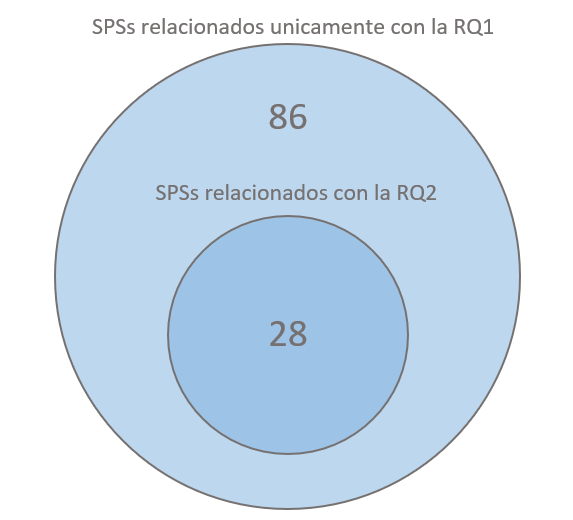
\includegraphics[scale=0.7]{resources/figures/Venn.png}
	\vspace{6pt}
	\caption{Relationship of SPSs with the research questions.}
	\label{fig:SPSsByRQs}
\end{figure}

Considering the relationships of the SPSs with the RQs, Figure \ref{fig:SPSsByRQs} shows that 100.00\% of the SPSs are related to RQ1, while 24.56\% of the SPSs are simultaneously related to both RQs. Consequently, the remaining 75.44\% are exclusively associated with RQ1. This indicates that no SPS is related solely to RQ2.

\begin{figure}[htbp]
	\centering
	\vspace{10pt}
	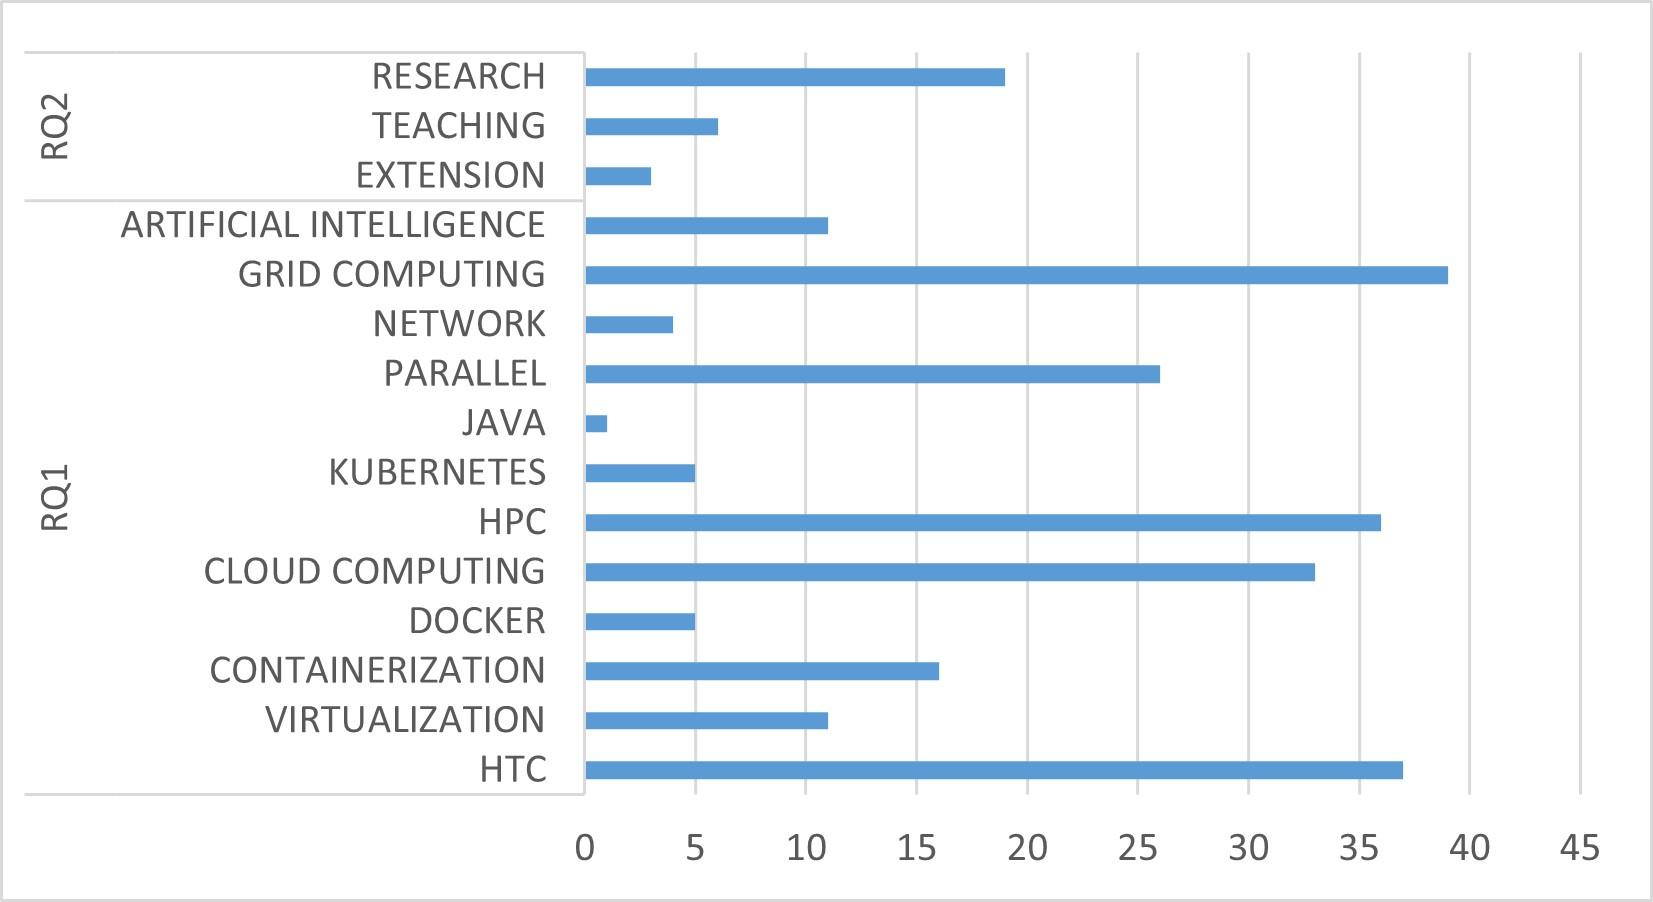
\includegraphics[scale=0.7]{resources/figures/SPSsByTopic.jpg}
	\vspace{6pt}
	\caption{Relationship of SPSs with research topics.}
	\label{fig:SPSsByTopics}
\end{figure}

Figure \ref{fig:SPSsByTopics} shows the topics defined during the planning stage for each research question and the number of SPSs inclusively associated with each topic. It is essential to note that one SPS may be linked to multiple topics simultaneously. In this sense, Figure \ref{fig:SPSsByTopics} displays the 14 topics associated with RQ1, where the topic ``Grid Computing'' is the most frequent at 34.21\%. In contrast, the least frequent topics are ``Java'' and ``Checkpointing,'' both at 0.87\%. On the other hand, Figure \ref{fig:SPSsByTopics} also shows the three topics associated with RQ2, where the topic ``Research'' is the most frequent at 16.67\%, while the least frequent is ``industry'' at 2.63\%.

\begin{figure}[htbp]
	\centering
	\vspace{10pt}
	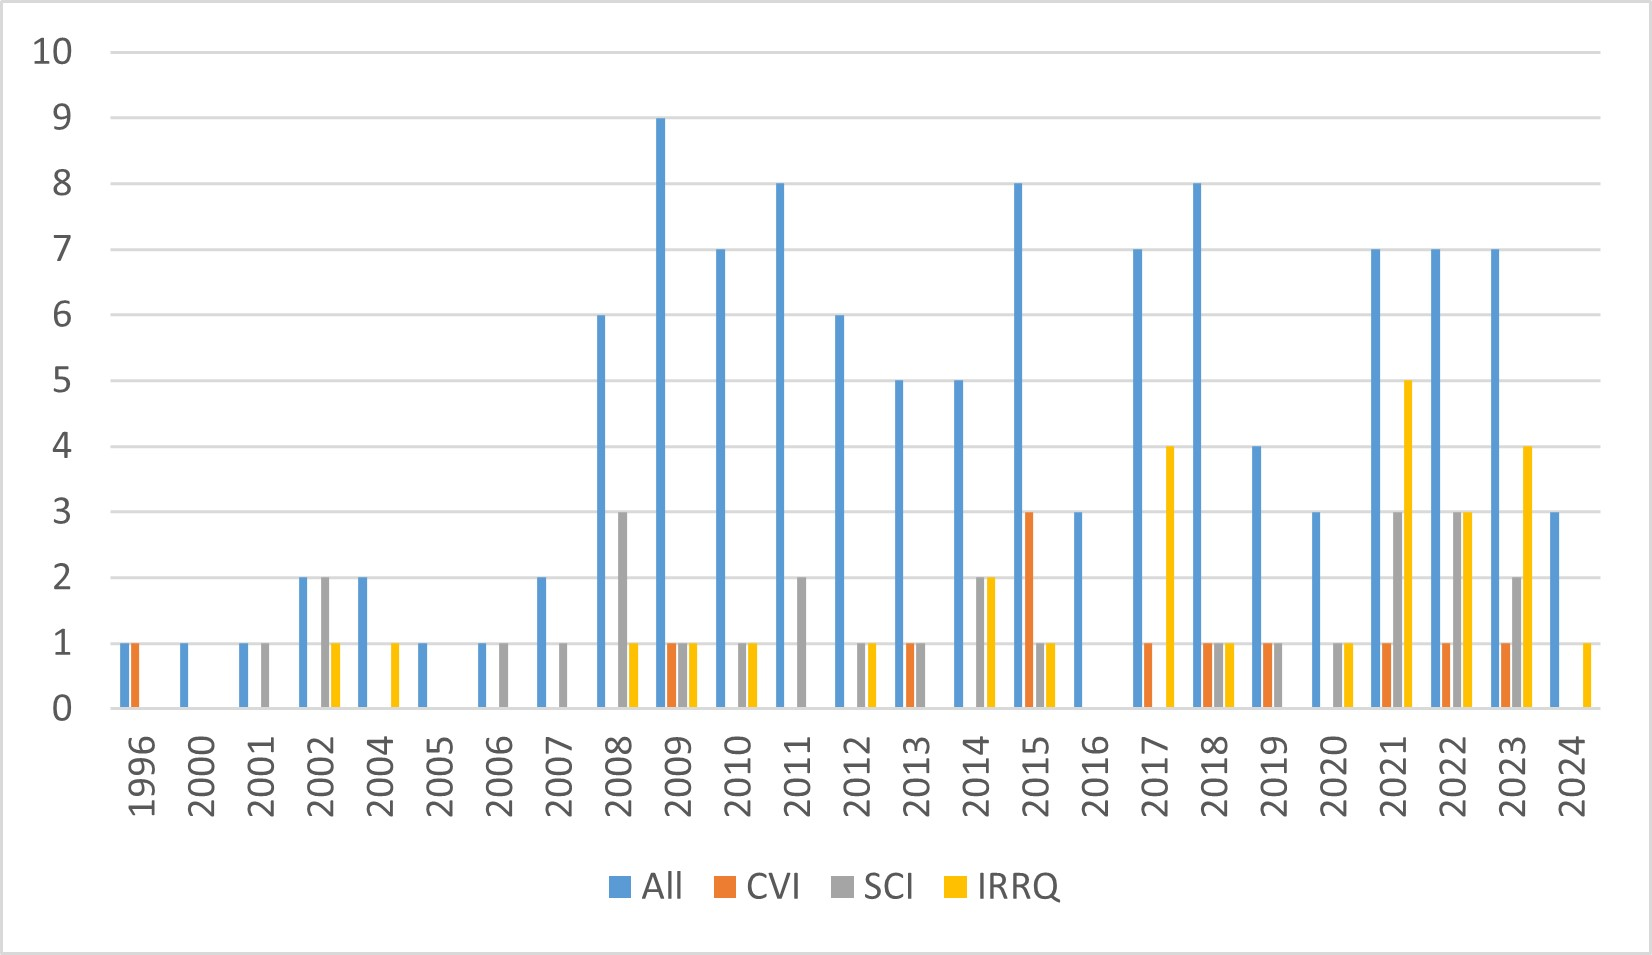
\includegraphics[scale=0.7]{resources/figures/SPSsBYearsAndIndexes.jpg}
	\vspace{6pt}
	\caption{Relationship of SPSs with years of publication and quality indices.}
	\label{fig:SPSsByYearsAndIndexes}
\end{figure}

The search period spans from 1996 to 2024. In this sense, Figure \ref{fig:SPSsByYearsAndIndexes} shows a low number of studies published between 1996 and 2007. In contrast, 2008 recorded an increase compared to 2007, with a total of 6 SPSs. The lowest number of SPSs was in 2009.

According to the SCI index, this SMS presents a relatively regular distribution across all years, with the exception of the period between 2006 and 2015, during which at least one SPS per year met the SCI index. Considering the distribution and the partially regular intervals in which no SPS met this index, this is regarded as an anomaly. Regarding the CVI index, the SMS shows regularity in the number of SPSs per year, particularly from 2017 onwards, except for the period between 2000 and 2008, when no SPS met the CVI index. Considering the IRRQ index, the year 2021 recorded the highest number of studies meeting this criterion, with a total of 5. Furthermore, there is evidence of a fairly consistent trend in the number of SPSs that satisfy this index over the years.

\begin{figure}[htbp]
	\centering
	\vspace{10pt}
	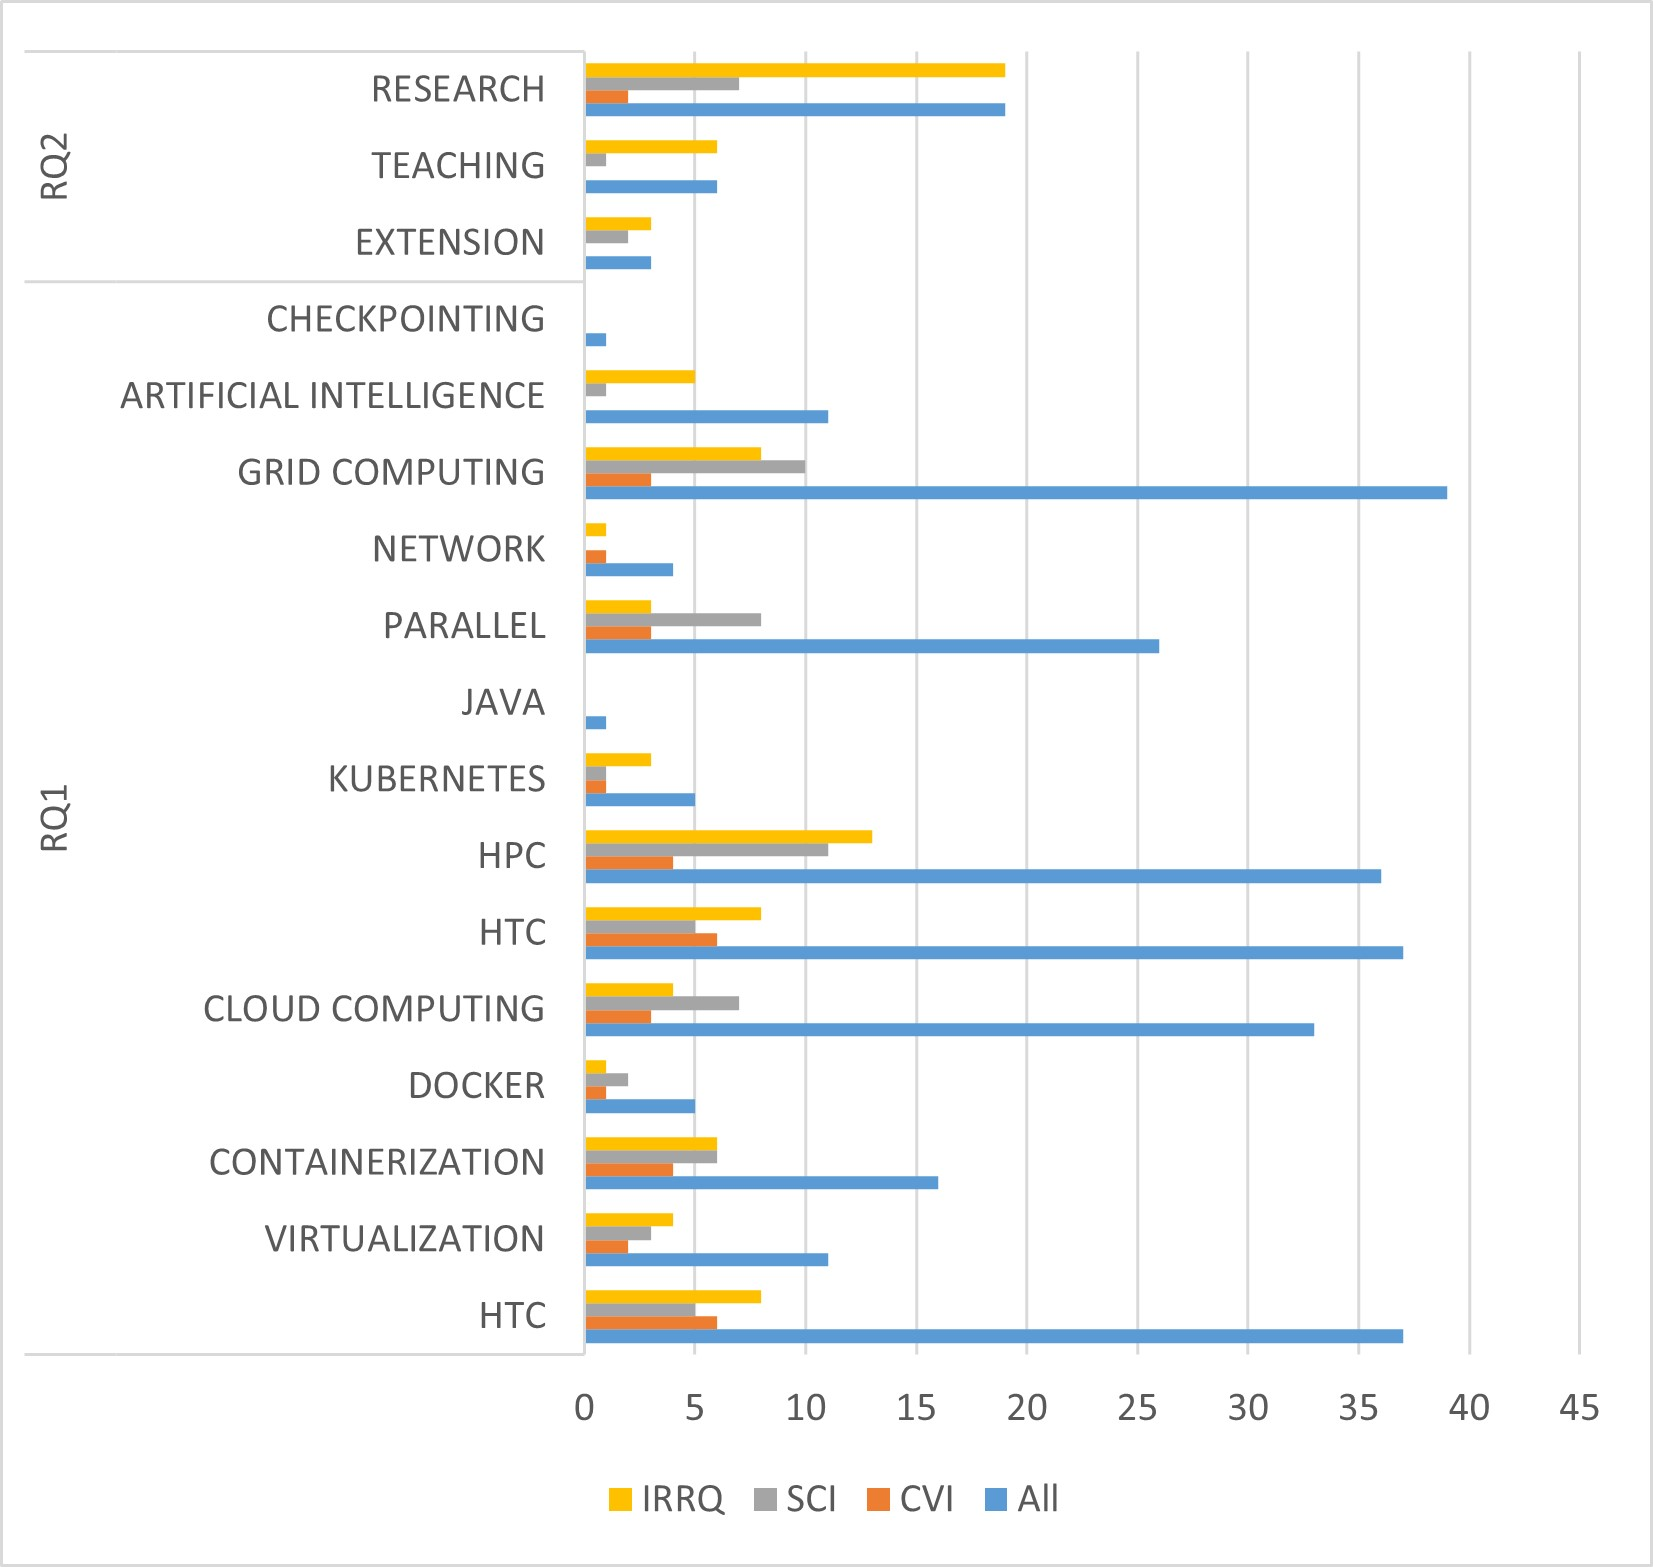
\includegraphics[scale=0.7]{resources/figures/IndexesByTopicAndRQs.jpg}
	\vspace{6pt}
	\caption{Quality indices by topic and research questions.}
	\label{fig:IndexesByTopicAndRQs}
\end{figure}

Figure \ref{fig:IndexesByTopicAndRQs} shows the number of SPSs classified by research question, including their respective topics and considering the quality indices.

In this sense, this study indicates that for RQ1, the topics ``Java'' and ``Checkpointing'' registered the lowest number with 1 SPS each, equivalent to 0.87\% of the 114 SPSs. In contrast, the topic ``Grid Computing'' is the most frequent with 39 SPSs, equivalent to 34.21\% of the 114 SPSs. On the other hand, for RQ2, the most frequent topic is ``Research,'' with 19 SPSs, equivalent to 16.66\% of the 114 SPSs. Conversely, the least frequent topic is ``industry,'' with 3 SPSs, equivalent to 2.63\% of the 114 SPSs.

With respect to the CVI, SCI, and IRRQ indices, we identified the topics ``Java,'' ``Checkpointing,'' and ``industry'' as the categories containing the fewest studies.

\begin{figure}[htbp]
	\centering
	\vspace{10pt}
	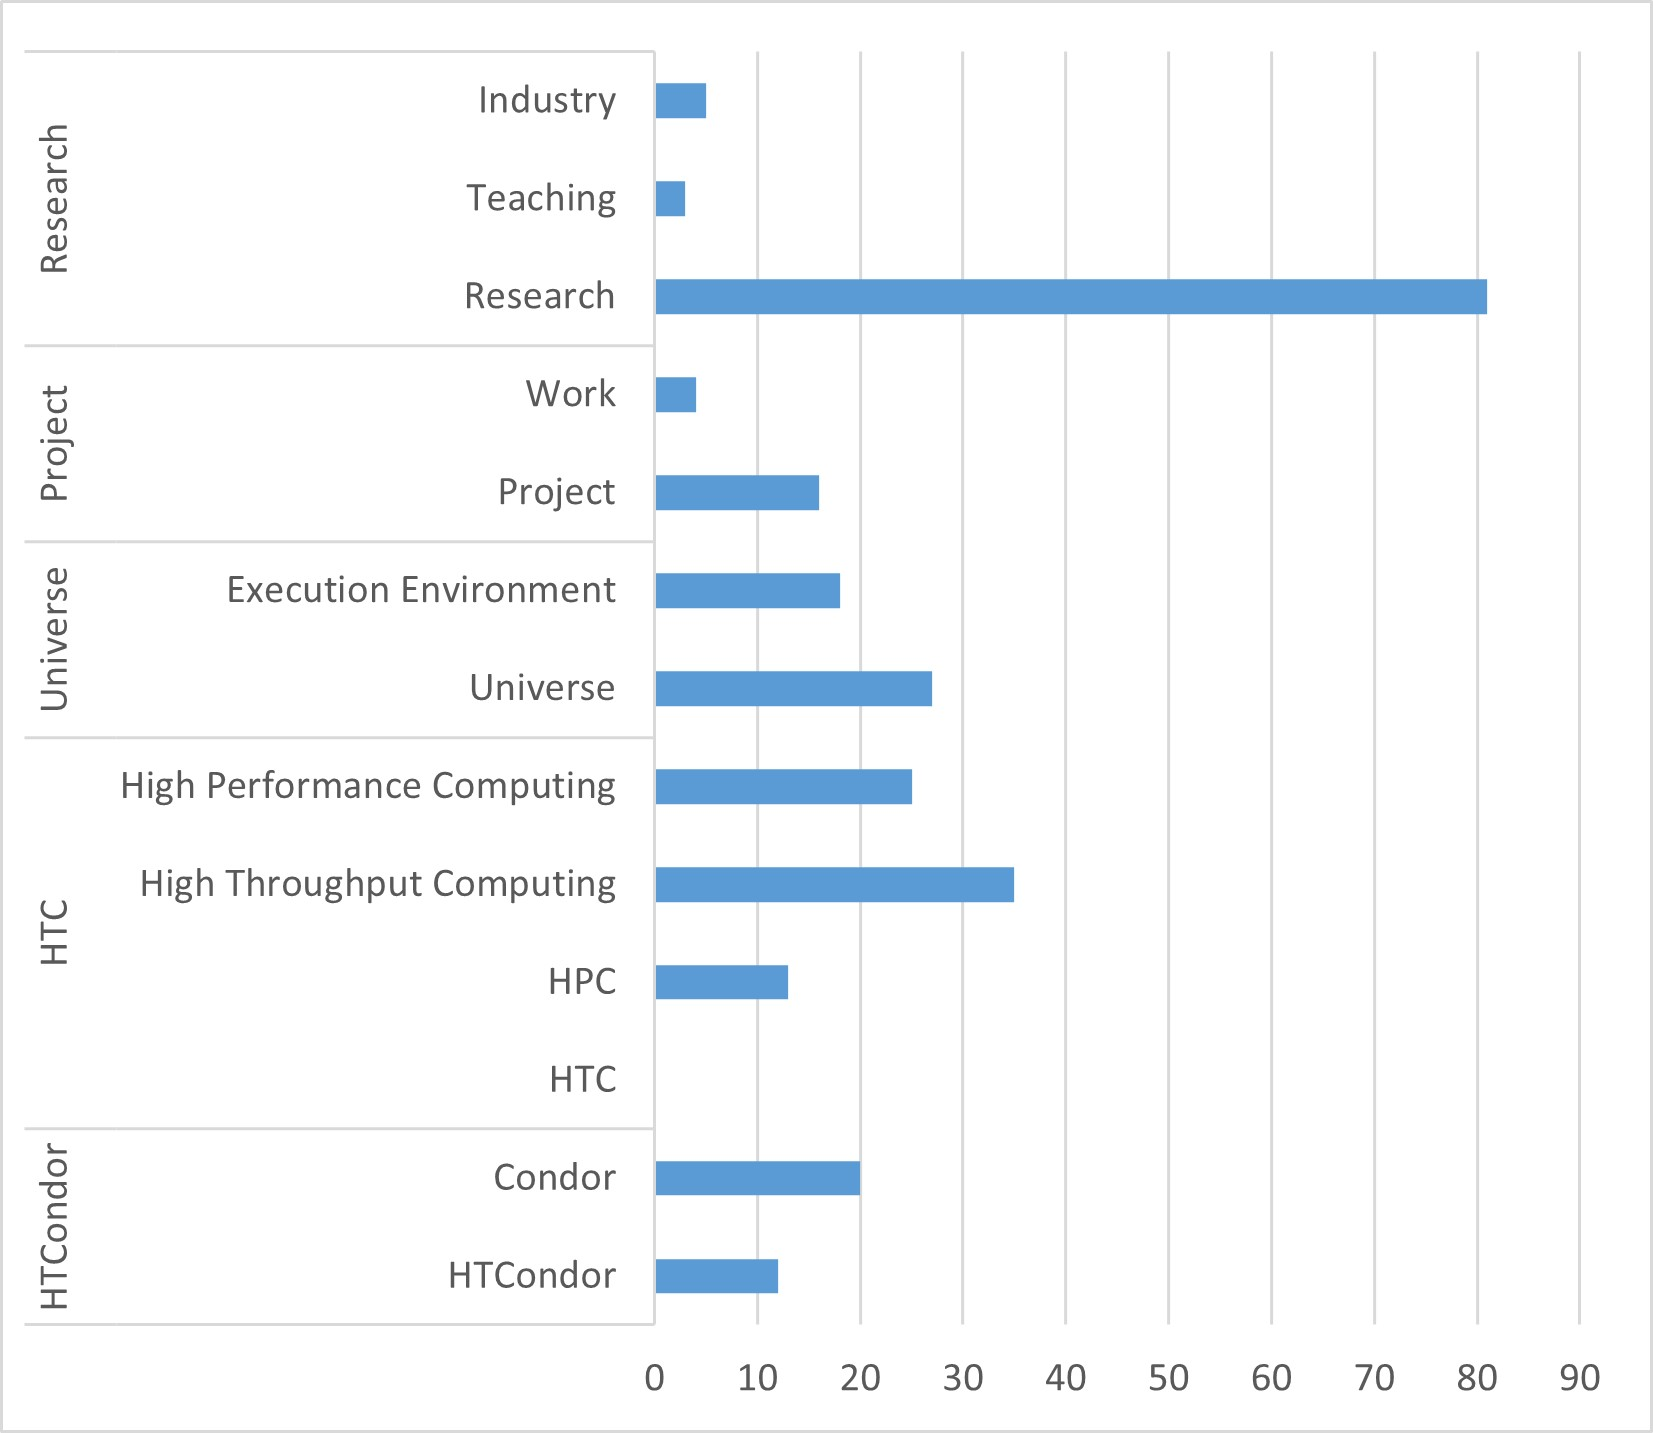
\includegraphics[scale=0.7]{resources/figures/SPSsByKeywords.jpg}
	\vspace{6pt}
	\caption{SPSs by keywords.}
	\label{fig:SPSsByKeywords}
\end{figure}

Figure \ref{fig:SPSsByKeywords} shows a cross-analysis between the SPSs, keywords, and synonyms. The synonym ``Work'' enabled the identification of 81 SPSs. Regarding the keyword ``Research,'' it led to the identification of 35 SPSs. In contrast, the keyword ``Universe'' made the smallest contribution, resulting in the identification of no SPSs.

% sub-subsection 4.6.2
\subsubsection{Word Cloud Visualization}

\begin{figure}[htbp]
	\centering
	\vspace{10pt}
	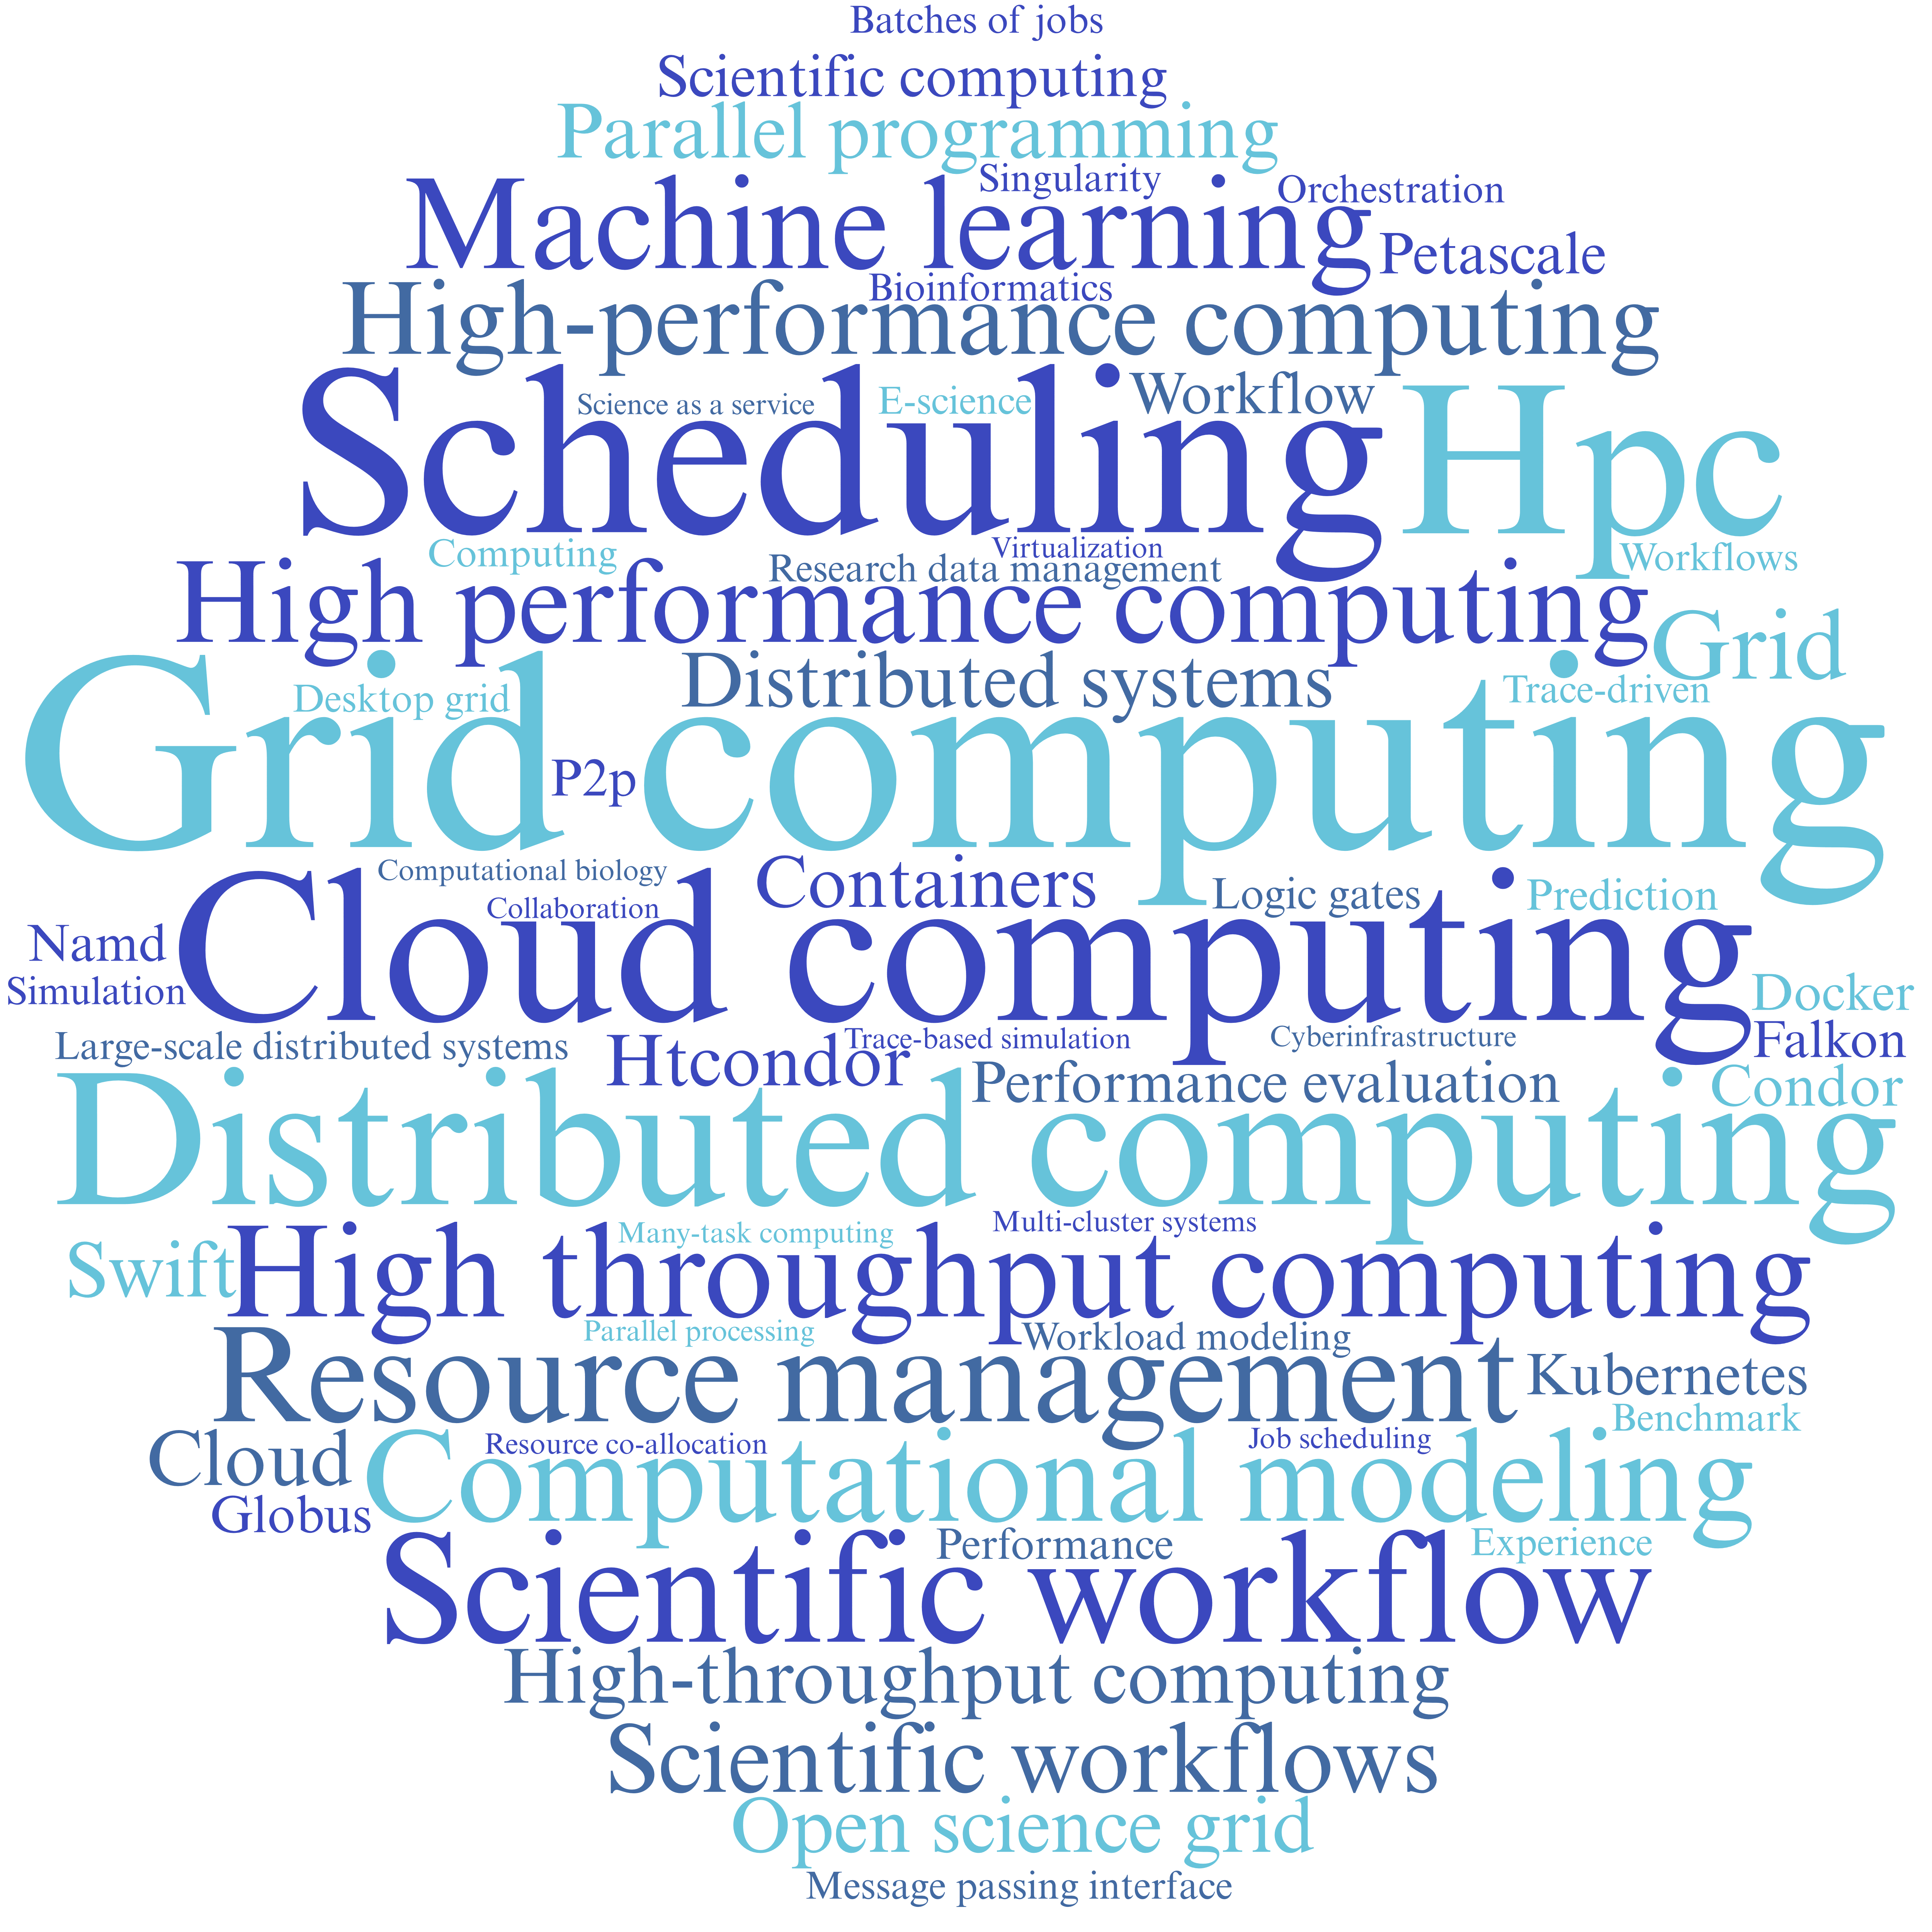
\includegraphics[scale=0.05]{resources/figures/wordcloud.png}
	\vspace{6pt}
	\caption{Word cloud of the keywords.}
	\label{fig:WordCloud}
\end{figure}

Another result obtained from the 114 SPSs of the SMS is the construction of a word cloud. This type of visualization seeks to highlight the most frequent and important words and concepts. Figure \ref{fig:WordCloud} shows the word cloud generated with the tool NubeDePalabras.es, built from the keywords of the SPSs.

Among the most frequent keywords, ``Cloud computing,'' ``Grid computing,'' and ``Distributed computing'' stand out, jointly contributing 18.59\% to the word cloud. The second level of relevance in terms of word cloud corresponds to ``HPC,'' ``High Throughput Computing,'' and ``Scheduling,'' contributing 11.98\%. Finally, a third level includes ``Resource Management,'' ``High Performance Computing,'' and ``Scientific workflow,'' contributing 7.85\%.

It should be emphasized that the calculations were made based on the words included in the cloud. In this case, all words with only one occurrence were excluded, so only words appearing at least twice were considered. This was done to extract the most relevant information. The percentages were then calculated based on the number of occurrences of the words with two or more appearances.
